\subtop{Algorithmus von Boyer und Moore}
\vspace*{-0.5\baselineskip}\begin{itemize}[itemsep=-1pt]
	\item die erwartete Laufzeit ist sublinear
	\item sehr gut in der praktischen Anwendung (vor allem bei Texten der natürlichen Sprache)
	\item \textbf{Idee:} der Vergleich von Pattern und Text startet beim letzten Zeichen des Patterns\\
		$\Rightarrow$ wenn das Zeichen aus dem Text, das mit dem letzten Zeichen des Patterns verglichen wird, nicht in $P$ vorkommt, müssen $m-1$ Zeichen nicht mehr betrachtet werden
\end{itemize}

\subsection{Bad Character Regel}
\vspace*{-0.5\baselineskip}\begin{itemize}[itemsep=-1pt]
	\item starten mit Vergleichen von $P[m]$ und $T[m+s]$
	\item Mismatch bei $j$ gefunden, das am weitesten rechts liegende Vorkommen des Elementes $x=T[s+j]$ in $P$ ist $k$\\
	$\Longrightarrow s$ kann erhöht werden um $j-k$
	\item wenn falls $k\geq j$ wird $s$ nur um $1$ erhöht (das am weitesten rechts liegende Vorkommen von $x$ liegt rechts der aktuellen Position, ist nicht optimal)\\
	$\Rightarrow$ Einführen der Funktion $r_P$ (das am weitesten rechts liegende Vorkommen eines Zeichens $a$ in $OP$):
		\begin{itemize}
			\item $\begin{array}[t]{rcl}
						r_P:\Sigma&\rightarrow&\{1,\dots,m\}\\
						a&\mapsto&\left\{\begin{array}{cl}
											0&\text{falls }a\text{ nicht in }P\text{ ist}\\
											\max\{j;P[j] = a\}& \text{sonst}
										\end{array}\right.
				\end{array}$
			\item falls das am weitesten rechts liegende Mismatch $=j$ gilt, wird die Verschiebung $s$ um\\
			$\max(1,j-r_P(T[s+j]))$ erhöht
		\end{itemize}
\end{itemize}
\subsection{Good Suffix Regel}
\vspace*{-0.5\baselineskip}\begin{itemize}[itemsep=-1pt]
	\item Mismatch bei $j=m-x$ mit $P[x,\dots,l]$ ist der am weitesten rechts liegende Teil-String von $P[1,\dots,m-1]$, der mit $P[j+1,\dots,m]$ übereinstimmend
	\item $s$ kann um $m-l$ erhöht werden
	\item die Funktion $s_P(j)$ ist die Länge des größten Präfixes von $P$, sodass eine der folgenden Eigenschaften gilt:
		\begin{enumerate}
			\item $P[j+1,\dots,m]$ ist ein Suffix von $P[1,\dots,s_P(j)]$ und $P[j] \neq P[s_P(j)-m+j]$\\\up
				\usetikzlibrary{positioning,patterns}

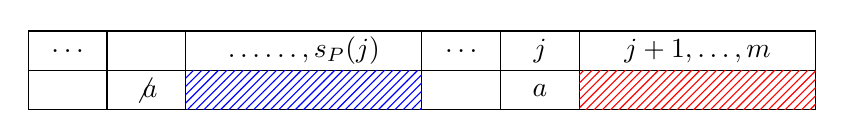
\begin{tikzpicture}[]

\draw(0,0)rectangle(10,1);
\draw(0,0)rectangle(10,0.5);

\foreach \x in {1,2,5,6,7}
	\draw(0,0)rectangle(\x,1);

\node at (0.5,.75) {$\dots$};
\node at (3.5,.75) {$\dots\dots,s_P(j)$};
\node at (5.5,.75) {$\dots$};
\node at (6.5,.75) {$j$};
\node at (8.5,.75) {$j+1,\dots,m$};

\node at (1.5,0.25) {$\not{a}$};
\node[pattern=north east lines,minimum height=0.5cm,minimum width=3cm,pattern color=blue] at (3.5,0.25) {};
\node at (6.5,0.25) {$a$};
\node[pattern=north east lines,minimum height=0.5cm,minimum width=3cm,pattern color=red] at (8.5,0.25) {};

\end{tikzpicture}
			\item[] oder
			\item $P[1,\dots,s_P(j)]$ ist ein Suffix von $P[j+1,\dots,m]$\\\up
				\usetikzlibrary{positioning,patterns}

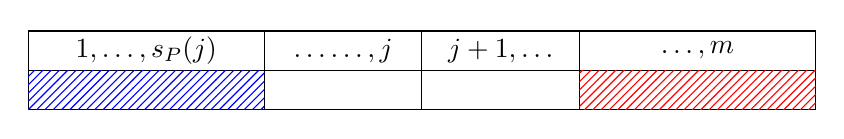
\begin{tikzpicture}[]

\draw(0,0)rectangle(10,1);
\draw(0,0)rectangle(10,0.5);

\foreach \x in {3,5,7}
	\draw(0,0)rectangle(\x,1);

\node at (1.5,.75) {$1,\dots,s_P(j)$};
\node at (4,.75) {$\dots\dots,j$};
\node at (6,.75) {$j+1,\dots$};
\node at (8.5,.75) {$\dots,m$};

\node[pattern=north east lines,minimum height=0.5cm,minimum width=3cm,pattern color=blue] at (1.5,0.25) {};
\node[pattern=north east lines,minimum height=0.5cm,minimum width=3cm,pattern color=red] at (8.5,0.25) {};

\end{tikzpicture}
			\item[]\begin{description}
				\item[Hinweis:] die roten und blauen Flächen können sich in den einzelnen Fällen überschneiden
				\end{description} 
		\end{enumerate}
	\item wenn das am weitesten rechts liegende Mismatch bei $j$ in $P$ auftaucht, kann die Verschiebung $s$ um $m-s_P(j)$ erhöht werden (\algo{Algorithmus von Boyer und Moore (mit \textcolor{red}{Galil-Erweiterung})}{\begin{algorithm}[H]
	\SetAlgoVlined
	\SetKwProg{Fn}{Function}{}{end}
	\KwIn{Text $T[1,\dots,n]$, Pattern $P[1,\dots,m]$ mit den Funktionen $r_P,s_P$}
	\KwOut{Verschiebungen $s$, an denen $P$ in $T$ vorkommt}
	\BlankLine
	\Begin{
		\textcolor{red}{$k\leftarrow 0$}\\
		$s\leftarrow 0$\\
		\While{$s\leq n-m$}{
			$j\leftarrow m$\\
			\While{$j>0$ \textcolor{red}{($j>k$)} und $P[j]=T[s+j]$}{
				$j\leftarrow j-1$
			}
			\eIf{$j>0$ \textcolor{red}{($j>k$)}}{
				\textcolor{red}{$k\leftarrow 0$}\\
				$s\leftarrow s+\max(m-s_P(j),j-r_p(T[s+j]))$
			}{
				output Verschiebung $s$\\
				\textcolor{red}{$k\leftarrow s_P(1)$}\\
				$s\leftarrow s+m-s_P(1)$
			}
		}
	}
\end{algorithm}})
	\item ist auch gut für große Alphabete
	\item \begin{description}
		\item[Laufzeit:]\ \\\up
			\begin{itemize}
				\item wenn nur die Good-Suffix-Regel angewendet wird, werden im schlechtesten Fall $3n-o(n)$ Vergleiche zwischen Zeichen ausgeführt
				\item Laufzeit ist nur dann sublinear, wenn die Bad-Character-Regel auch angewendet wird
				\item allgemein: $\Theta(m(n-m+1))$ (z.B. $T=a^n,P=a^m$)
				\item mit der Erweiterung von Galil: linear
				\item die Modifikation verhindert das vergleichen von schon bekannten Teil-Zeichenketten (wobei $s_P(j)=\pi(m)$)
			\end{itemize}
	\end{description}
\end{itemize}
\subsection{Vorverarbeitung}
\subsubsection*{Bad Character Regel}
\begin{itemize}[itemsep=0pt]
	\item $r_P$ kann in $\BigO(m+|\Sigma|)$ berechnet werden ($r_P(P[j])\leftarrow j,~~\forall j=1,\dots m$)
	\item durch Speichern aller Vorkommnisse eines Zeichens in $P$ von links nach rechts anstatt nur dem rechtesten Vorkommens, kann die Erhöhung der Verschiebung größer sein, da man dann auch eine größere Verschiebung hat, falls das rechteste Vorkommen links des Mismatches liegt
	\item Worst-Case-Laufzeit: höchstens verdoppelt
\end{itemize}

\subsubsection*{Good Suffix Regel}
\begin{itemize}[itemsep=-2pt]
	\item Aufteilen der Berechnung von $s_P$ in zwei Teile mit $\max\emptyset=0$:
		\begin{description}
			\item[$s_P^{match}(j)$] $= \max\{m-j+1\leq k<m;P[j+1,\dots,m]\text{ ist Suffix von }P[1,\dots,k]\text{ und }P[j]\neq P[k-m+j]\}$
			\item[$s_P^{pref}(j)$] $=\underbrace{\max\{0\leq k<m;P[1,\dots,k]\text{ ist Suffix von } P[j+1,\dots,m]\}}_{=\text{suf}_P(P[j+1,\dots,m])}$
		\end{description}
	\item $s_P(j)=\max(s_P^{match}(j),s_P^{pref}(j))$
	\item Berechnung von $s_P^{pref}$:
		\begin{enumerate}
			\item $\pi$ ist die \bound~des Knuth-Morris-Pratt-Matcher
			\item $s_P^{pref}$ ist die Länge der größten Begrenzung von $P$, dessen Länge höchstens $m-j$ ist
			\item die Begrenzungen von $P$ sind genau die Suffixe von $P$ der Länge $m,\pi(m),\pi^2(m),\dots,0$\\
			$\Rightarrow s_P^{pref}=\pi^k(m) \Longleftrightarrow\pi^k(m)\leq m-j<\pi^{k-1}(m)$\\\up
			\usetikzlibrary{positioning,patterns,decorations.pathreplacing}

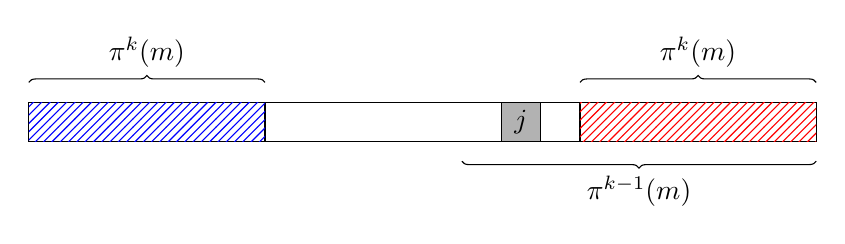
\begin{tikzpicture}[]

\draw(0,0)rectangle(10,0.5);
\node[fill=black!30,minimum height=0.5cm,minimum width=0.5cm] at (6.25,0.25) {};
\foreach \x in {3,6,6.5,7}
	\draw(0,0)rectangle(\x,0.5);

\node[pattern=north east lines,minimum height=0.5cm,minimum width=3cm,pattern color=blue] at (1.5,0.25) {};
\node at (6.25,0.25) {$j$};
\node[pattern=north east lines,minimum height=0.5cm,minimum width=3cm,pattern color=red] at (8.5,0.25) {};

\draw decorate [decoration={name=brace},thick]  {(0,0.75) -- node[above=0.4ex] {$\pi^k(m)$}  (3,0.75)};
\draw decorate [decoration={name=brace},thick]  {(7,0.75) -- node[above=0.4ex] {$\pi^k(m)$}  (10,0.75)};
\draw decorate [decoration={name=brace},thick]  {(10,-0.25) -- node[below=0.4ex] {$\pi^{k-1}(m)$}  (5.5,-0.25)};

\end{tikzpicture}
		\vspace*{-0.5\baselineskip}\item[$-$] somit kann $s_P^{pref}$ in $\BigO(m)$ berechnet werden (\algo{Good Suffix Regel (Prefix-Fall)}{arg2})
		\end{enumerate}
	\item Berechnung von $s_P^{match}$:
		\begin{enumerate}
			\item Grundlage: Berechnung von $\pi$\\
				zur Erhöhung von $i$, wird nach dem größten Präfix $P[1,\dots,q]$ von $P$ gesucht, das ein Suffix von $P[2,\dots,i-1]$ ist und für das gilt $P[i]=P[q+1]$
			\item da die Präfixe von $P$, die Suffixe von $P[2,\dots,i-1]$ sind, all die Präfixe der Länge\\
				$\pi(i-1),\pi^2(i-1),\dots,0$ sind, müssen alle Präfixe dieser Länge geprüft werden, bis die Bedingung $P[i]=P[q+1]$ erfüllt ist\\\up
				\usetikzlibrary{positioning,patterns,decorations.pathreplacing}

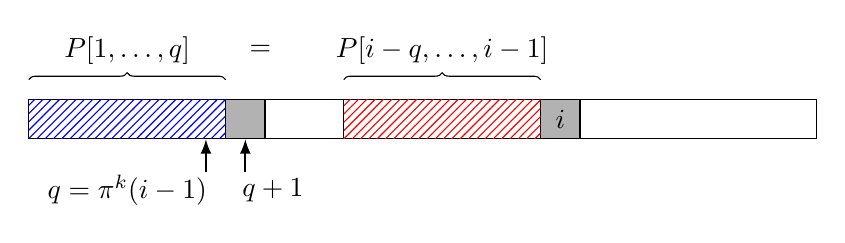
\begin{tikzpicture}[]

\draw(0,0)rectangle(10,0.5);
\node[fill=black!30,minimum height=0.5cm,minimum width=0.5cm] at (6.75,0.25) {};
\node(0)[fill=black!30,minimum height=0.5cm,minimum width=0.5cm] at (2.75,0.25) {};
\foreach \x in {2.5,3,4,6.5,7}
	\draw(0,0)rectangle(\x,0.5);

\node[pattern=north east lines,minimum height=0.5cm,minimum width=2.5cm,pattern color=blue] at (1.25,0.25) {};
\node at (6.75,0.25) {$i$};
\node[pattern=north east lines,minimum height=0.5cm,minimum width=2.5cm,pattern color=red] at (5.25,0.25) {};

\node(1)[xshift=.35cm] at (2.75,-.65) {$q+1$};
\node(1)[rotate=-90] at (2.75,-.55) {};
\node(2)[xshift=-1cm] at (2.25,-.65) {$q=\pi^k(i-1)$};
\node(2)[rotate=-90] at (2.25,-.55) {};
\node(3)[minimum height=0.5cm,minimum width=0.5cm] at(2.25,0.25){};

\draw[-latex,thick](1)to(0);
\draw[-latex,thick](2)to(3);
\draw decorate [decoration={name=brace},thick]  {(0,0.75) -- node(0)[above=0.4ex] {$P[1,\dots,q]$}  (2.5,0.75)};
\draw decorate [decoration={name=brace},thick]  {(4,0.75) -- node[above=0.4ex] {$P[i-q,\dots,i-1]$}  (6.5,0.75)};

\node[right=of 0,xshift=-0.5cm]{$=$};
\end{tikzpicture}
		\end{enumerate}
	\item Berechnung von $\oben{\pi}$ (\bound~des umgekehrten Patterns $P[m,\dots,1]$):
		\begin{itemize}[itemsep=-2pt]
			\item im Algorithmus müssen alle $P[j],~j=1,\dots,m$ durch $P[m-j+1]$ ersetzt werden, sowie Prefix und Suffix in der Beschreibung
			\item immer wenn der Test $P[m-i+1]\overset{?}{=}P[m-q]$ fehlschlägt, weiß man, dass $P[m-q+1,\dots,m]=P[m-i+2,\dots,m-i+1+q]$ sowie $P[m-q]\neq P[m-i+1]$ gilt\\\up
			\usetikzlibrary{positioning,patterns,decorations.pathreplacing}

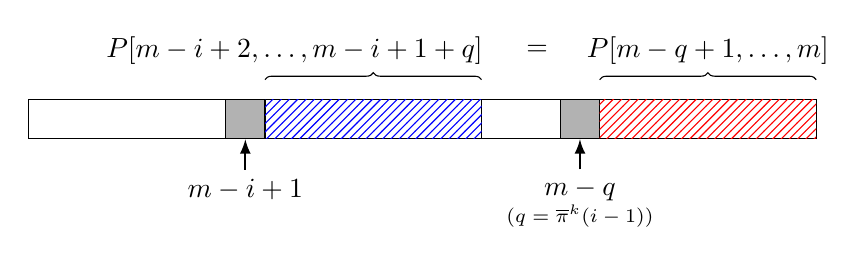
\begin{tikzpicture}[node distance=-0.2cm]

\draw(0,0)rectangle(10,0.5);
\node(3)[fill=black!30,minimum height=0.5cm,minimum width=0.5cm] at (7,0.25) {};
\node(0)[fill=black!30,minimum height=0.5cm,minimum width=0.5cm] at (2.75,0.25) {};
\foreach \x in {2.5,3,5.75,6.75,7.25}
	\draw(0,0)rectangle(\x,0.5);

\node[pattern=north east lines,minimum height=0.5cm,minimum width=2.75cm,pattern color=blue] at (4.375,0.25) {};
\node[pattern=north east lines,minimum height=0.5cm,minimum width=2.75cm,pattern color=red] at (8.625,0.25) {};

\node(1) at (2.75,-.65) {$m-i+1$};
\node(2) at (7,-.65) {$m-q$};
\node(21)[below=of 2]{\scriptsize$(q=\overline{\pi}^k(i-1))$};
%\node(2)[rotate=-90] at (2.25,-.55) {};
%\node(3)[minimum height=0.5cm,minimum width=0.5cm] at(2.25,0.25){};

\draw[-latex,thick](1)to(0);
\draw[-latex,thick](2)to(3);
\draw decorate [decoration={name=brace},thick]  {(3,0.75) -- node(0)[above=0.4ex,xshift=-1cm] {$P[m-i+2,\dots,m-i+1+q]$}  (5.75,0.75)};
\draw decorate [decoration={name=brace},thick]  {(7.25,0.75) -- node[above=0.4ex] {$P[m-q+1,\dots,m]$}  (10,0.75)};

\node[right=of 0,xshift=0.5cm]{$=$};
\end{tikzpicture}
		\end{itemize}
\end{itemize}
\topbreak
\up\up
\begin{itemize}
	\item[]
		\begin{itemize}
			\item somit gilt $s_P^{match}\geq m-i+1+q$ (\algo{Good Suffix Regel (Matching-Fall)}{arg2})
			\item das beinhaltet die Idee zr Berechnung von $s_P^{match}$ in $\BigO(m)$
			\item bleibt zu zeigen, dass der Algorithmus richtig arbeitet:
				\begin{enumerate}
					\item explizites Setzen von $s_P^{match}(m)$ (notwendig, weil die While-Schleife bei $q=0$ nicht durchläuft)
					\item $j=1,\dots,m-1$, sodass $s_P^{match}(j)\neq 0$ und $i=1,\dots,m$, sodass $m-i+1=s_P^{match}(j)-(m-j)$\\\up
						\usetikzlibrary{positioning,patterns,decorations.pathreplacing}

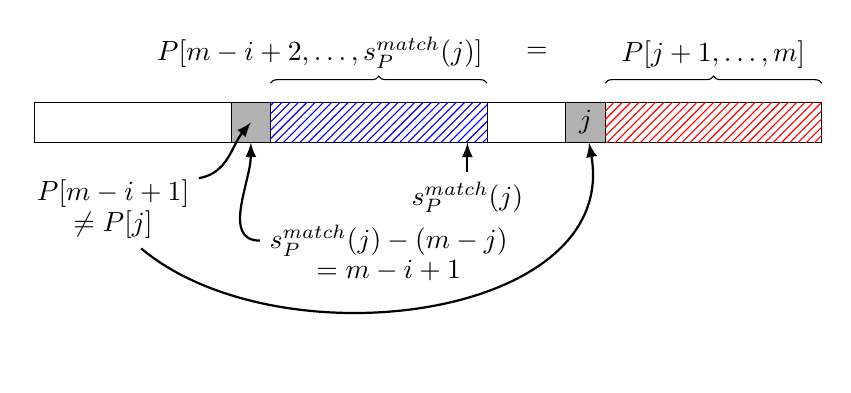
\begin{tikzpicture}[node distance=-0.2cm]

\draw(0,0)rectangle(10,0.5);
\node(3)[fill=black!30,minimum height=0.5cm,minimum width=0.5cm] at (7,0.25) {};
\node(0)[fill=black!30,minimum height=0.5cm,minimum width=0.5cm] at (2.75,0.25) {};
\foreach \x in {2.5,3,5.75,6.75,7.25}
	\draw(0,0)rectangle(\x,0.5);

\node[pattern=north east lines,minimum height=0.5cm,minimum width=2.75cm,pattern color=blue] at (4.375,0.25) {};
\node[pattern=north east lines,minimum height=0.5cm,minimum width=2.75cm,pattern color=red] at (8.625,0.25) {};

\node[xshift=1.75cm](1) at (2.75,-1.25) {$s_P^{match}(j)-(m-j)$};
\node(12)[below=of 1]{$=m-i+1$};
\node(2) at (1,-.65) {$P[m-i+1]$};
\node(21)[below=of 2]{$\neq P[j]$};
\node(5)[] at (5.5,-.7) {$s_P^{match}(j)$};
\node(4)[minimum height=0.5cm,minimum width=0.5cm] at (5.5,0.25) {};
\node[] at(3){$j$};

\draw[-latex,thick](1)to[out=180,in=270](0);
\draw[-latex,thick](5)to(4);
\draw[-latex,thick](21)to[out=-40,in=280](3);
\draw[-latex,thick](2)to[out=10,in=230](0.center);

\draw decorate [decoration={name=brace},thick]  {(3,0.75) -- node(0)[above=0.4ex,xshift=-0.75cm] {$P[m-i+2,\dots,s_P^{match}(j)]$}  (5.75,0.75)};
\draw decorate [decoration={name=brace},thick]  {(7.25,0.75) -- node[above=0.4ex] {$P[j+1,\dots,m]$}  (10,0.75)};

\node[right=of 0,xshift=0.5cm]{$=$};
\end{tikzpicture}
					\item aus $P[j+1,\dots,m]$ ist eine Begrenzung von $P[m-i+2,\dots,m-1]$ folgt, dass es ein $k$ geben muss, sodass $j=m-\oben{\pi}^k(i-1)$
					\item zu Zeigen: der Algorithmus hat höchstens $k$ Iterationen pro For-Schleifen-Durchlauf $i$
					\item wenn (4) nicht wahr wäre, gäbe es ein $q=\oben{\pi}^{k'}(i-1) > \oben{\pi}^k(i-1)$ mit $P[m-q]=P[m-i+1]$\\
					es gilt aber: $P[m-i+1]\neq P[j]$ somit gilt: $m-q+(m-j)$ erfüllt alle Bedingungen für $s_P^{match}(j)$, ist aber größer als $s_P^{match}(j)\\
					\Rightarrow$ Widerspruch
				\end{enumerate}
		\end{itemize}
\end{itemize}